\subsection{Formalization of consistency guarantees}

\begin{definition}{Stream processing system}
is a tuple of $(\Gamma,D,W)$, where $\Gamma$ is all possible data flow elements, $D$ is dependency relation between elements, and $W$ is a set of elements in a system. 
\end{definition}

\begin{definition}{Dependency relation}
$D\subseteq{\Gamma\times\Gamma}$ is a binary relation. Pair $(x,y)\in{D}$ iff $y$ can be generated from $x$ within logical graph operations.
\end{definition}

Let $\tau\in{\mathbb{N}}$ be an exact global discrete time. Let $a_\tau\in{\Gamma}$ be the element, which enters at the time $\tau$, and $b_\tau\in{\Gamma}$ is the element, which leaves at the time $\tau$. 

\begin{definition}{Working set}
$W_\tau\subseteq{\Gamma}$ at the time $\tau$ is the set of elements, which are currently in the system:

$W_0=\emptyset$:

$W_{\tau+1}=\begin{sqcases}
W_{\tau}\cup{a_\tau}, & \text{or}\\
W_{\tau}\setminus{b_{\tau+1}}, & \text{or}\\
W_{\tau}\setminus{X}\cup{Y}, \forall{x\in{X}\exists{y\in{Y}}}:(x,y)\in{D} & \text{}.
\end{sqcases}$

\end{definition}

We can imagine a stream processing system as a pool, where some elements are poured in and others are poured out. Inside a pool, each element can be substituted by the other element, which can be substituted as well, and so on. Only survived elements are poured out from the pool.

In terms of proposed definitions, we can declare any state-of-the-art stream processing system. In Storm, $\Gamma$ contains all possible {\em Tuples}, while in Flink all {\em StreamRecords}. The notion of dependency $D$ expresses two possible scenarios. The first one is a transformation into other elements due to, e.g., {\em Bolts} in Storm or {\em Operators} in Flink. In this case, transformed elements depend on original ones. The second option is combining an element and a {\em state} into the new state. It implies that the new state depends on the previous state and the element. In both Storm and Flink, a state can be managed using state handlers, e.g., {\em KeyValueState} in Storm and {\em ValueState} in Flink. Technically, states in these systems are not data flow elements, but as it was mentioned above, they can be considered as data flow elements.

Regarding dependencies, we can draw an analogy with {\em Herbrand semantics}, where the binary relation is used to express, which write operations affect the read operation.

Let $A_{\infty}=\bigcup\limits_{i=1}^{\infty}{a_i}$ be a set of all input elements.

\begin{definition}{System state}
$S_\tau$ at the time $\tau$ is $W_\tau^{\infty}$ if $A_{\infty}=\bigcup\limits_{i=1}^{\tau}{a_i}$.
\end{definition}

\begin{definition}{Nullification time}
of an input element $a_\tau$ is the time $\theta_{a_\tau}=inf(\hat{\tau}>\tau|W_{\hat{\tau}}\setminus{S_{\hat{\tau}}}\cap{Cl(D)(a_\tau)=\emptyset})$, where $Cl(D)$ is a transitive closure of the relation $D$.
\end{definition}

The main purpose of the state is to accumulate the information about input items. Data flow elements cannot be in $W\setminus{S}$ for an infinite time by the definition. Hence, for each input element $a_\tau$, there is a nullification time $\theta_{a_\tau}$, thereafter all elements, which depend on $a_\tau$, are in the system state. Since the nullification time, the input element can affect output elements only through the state. The concept of nullification is shown in Figure~\ref{nullification}. 

\begin{figure}[htbp]
  \centering
  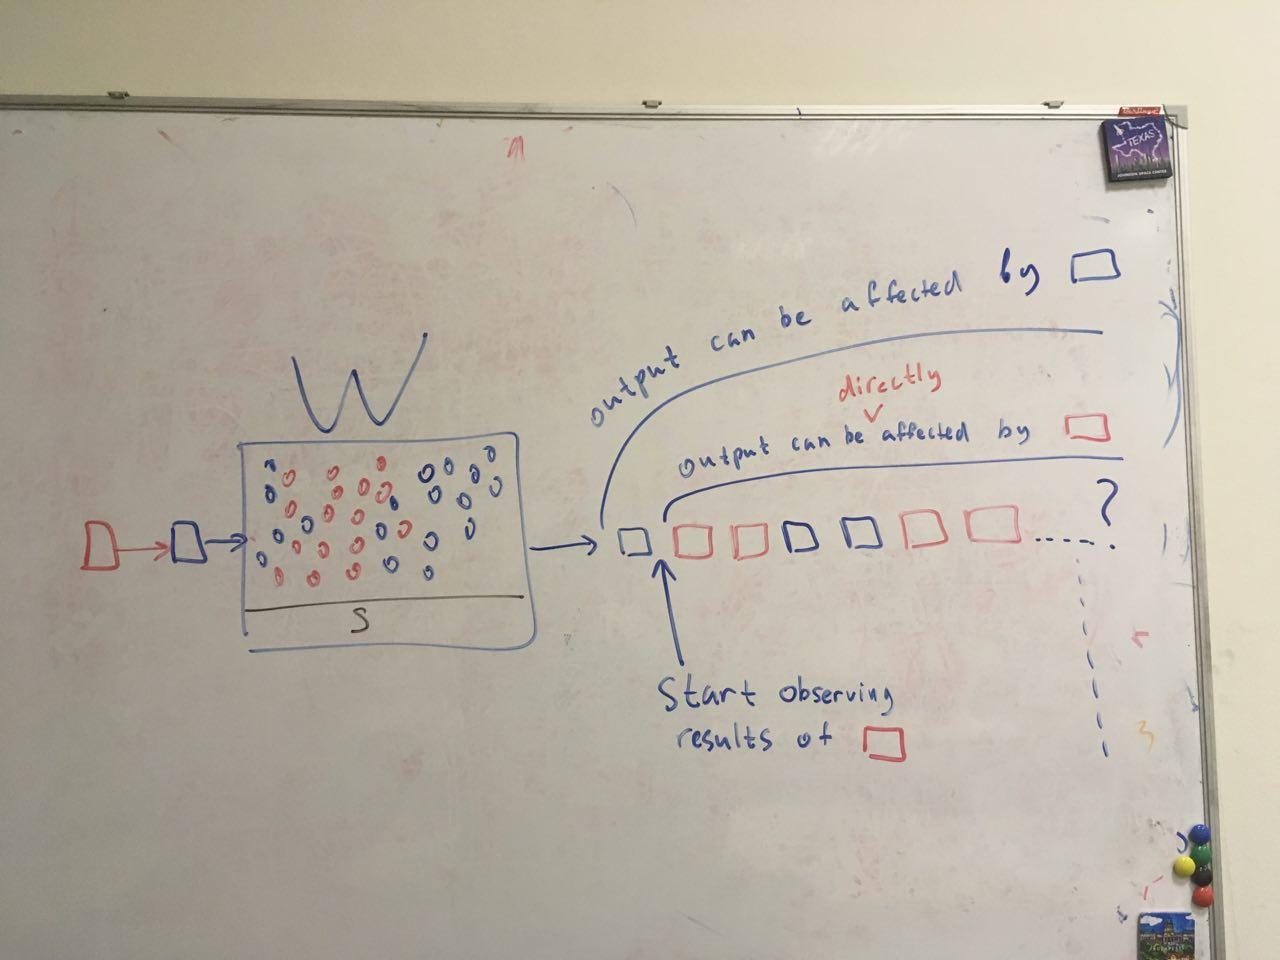
\includegraphics[width=0.48\textwidth]{pics/nullification}
  \caption{The red and blue elements have entered the system. Since that time, it is unclear, when they stop directly affect output elements}
  \label {nullification}
\end{figure}

\begin{definition}{Time quantization}
$t$ is the time of input, output, and nullification:

$t=\begin{cases}
\tau_i:\exists{a_{\tau_i}}, \\
\tau_o:\exists{b_{\tau_o}}, \\
\theta_{a_\tau}:\forall{a_\tau}.
\end{cases}$
\end{definition}

Time quantization allows us to consider only {\em observable} points in time. The time of input and output elements is obviously observed by any system. The mechanisms for tracking nullification vary slightly more. In Storm, a special agent called {\em Acker} is used. In Flink, nullification time is tracked using {\em low watermarks}. In Spark Streaming nullification time for each element in a micro-batch coincides with the time, when the micro-batch is fully processed.

Let $x,a^{1},a^\infty$ be input elements with arbitrary arrival times. $\mathbb{B}_t$ are all output elements by the time $t$:

$\mathbb{B}_t=\bigcup\limits_{i=1}^{t}{b_i}$

Let $p(W_t,\mathbb{B}_t|x,a^{1}...a^\infty)$ be a probability to observe working set $W_t$ and output elements $B_t$ at the time $t$ if input elements are $x,a^{1},a^\infty$. Let us construct three sets:

$X^0=(W_\infty,\mathbb{B}_\infty|p(W_\infty,\mathbb{B}_\infty|a^{1}...a^\infty)\neq{0})$

$X^1=(W_{\theta_{x}},\mathbb{B}_{\theta_{x}}|p(W_{\theta_{x}},\mathbb{B}_{\theta_{x}}|x,a^{1}...a^\infty)\neq{0},\forall{i}:{a^i}\neq{x})$

$X^{*}=(W_{\theta_{x}},\mathbb{B}_{\theta_{x}}|p(W_{\theta_{x}},\mathbb{B}_{\theta_{x}}|x,a^{1}...a^\infty)\neq{0},\\
\exists{i}:{a^i={x}},\exists{y:y\in{W_{\theta_{x}}\setminus{S_{\theta_x}}}\cap{Cl(D)(a^i)}})$

These sets model the {\em observable} output, current elements, and state of a stream processing engine. $X^0$ expresses the case, when element $x$ has not affected the system, so it is a forbidden behavior for at least once and exactly once guarantees. On the other hand, $X^{*}$ defines possible results, after $x$ has been nullified, but $a^i=x$ or its dependencies are in the system. Such behavior can cause inconsistencies in system state due to duplicates and should not be observed if the system provides for at most once or exactly-once. Using these modeled sets now we can define guarantees.

\begin{definition}{At most once}
guarantee is provided by a system iff $\forall{x,a^{1}...a^\infty}:X^{1}\cap{X^{*}}=\emptyset$
\end{definition}

\begin{definition}{At least once}
guarantee is provided by a system iff $\forall{x,a^{1}...a^\infty}:X^{0}\cap{X^{1}}=\emptyset$
\end{definition}

\begin{definition}{Exactly once}
guarantee is provided by a system iff $\forall{x,a^{1}...a^\infty}:X^{1}\cap{X^{*}}=\emptyset \wedge X^{0}\cap{X^{1}}=\emptyset$
\end{definition}

% Now streaming consistency guarantees are defined in terms of correspondences between input, output and the system state. Custom system or user-defined semantics are not considered in this model, e.g., if the system drops all input items, it also can be claimed as supporting exactly-once. Looking from another side, our model formally describes which properties are {\em exactly} supported by state-of-the-art stream processing systems, such as Flink, Storm, Spark Streaming, Samza, MillWheel, etc, so we can discuss its properties in unified terms.

We defined streaming consistency guarantees in terms of the proposed model. This model is suitable for state-of-the-art stream processing systems, such as Flink, Storm, Spark Streaming, Samza, MillWheel, etc, so now we can discuss its properties in unified terms.

\subsection{Implementation properties and notes}

% In this section, we formally define some additional concepts and demonstrate a potential way to reduce latency overhead on consistency guarantees. We mainly consider exactly once, because it is the strongest guarantee, which is extremely valuable in practice.    

\begin{definition}{System failures}
are the time moments, when the system loses its working set. 
\end{definition}

Assume that the system fails at time $\tau_f$. The naive idea for recovering is to simply start processing from the very beginning, i.e., to set $W_{\tau_f+1}=\emptyset$ and to replay the whole input stream. However, storing and replaying the whole input stream is inefficient in terms of both memory and time consuming and can violate consistency guarantees.

\begin{definition}{Snapshot}
at time $\tau_s$ is persistently stored $P_{\tau_s}\subseteq{W_{\tau_s}}$ that is not lost even in case of failure.
\end{definition}

Snapshots allow a system to restart processing since defined points. One approach for taking snapshots is to save (or update) the whole $W_{\tau}$ on each $\tau$. In this case, there is no need to replay input elements, because the system can completely restore computations using only a snapshot. Google MillWheel uses this method for recovering. {\em Strong productions} mechanism allows MillWheel to preserve exactly-once guarantee for the price of persistent updates of $P_\tau=W_\tau$ on each $\tau$~\cite{Akidau:2013:MFS:2536222.2536229}.    

Another approach is to take so-called {\em state snapshots}. This kind of snapshots is considered in practice only within the time quantization $t$. It assumes that $\forall{t_s}:P_{t_s}=S_{t_s}$ and requires replay of input element. Suppose, there is a state snapshot at time $t_s$ and a system fails at time $\tau_f>t_s$. In order to recover processing, system sets $W_{\tau_f+1}=P_{t_s}$ and requests for replay elements $a$ such that $\forall{y\in{Cl(D)(a)}}:y\notin{P_{t_s}}$. The idea of taking snapshots is illustrated in Figure~\ref{snapshotting}.

\begin{definition}{Consistent state snapshot}
$P^{c}_{t_s}=S_{t_s}$ at time $t_s$ is a snapshot such that $\forall{a}\in{Cl^{-1}(D)(P^{c}_{t_s})}:\exists{\theta_a}$.
\end{definition}

\begin{theorem}
A system, that uses state snapshots for recovery, provides for at most once guarantee only if all state snapshots are consistent.  
\end{theorem}

Our notion of consistent state snapshot modifies the classical definition of {\em consistent distributed snapshot} proposed in~\cite{Chandy:1985:DSD:214451.214456} for the case where dependencies between messages exist and input element must be applied to state atomically with its inversed dependencies. This notion is natural for stream processing systems because as it was shown, it is directly connected with streaming consistency guarantees. 

One popular method for taking consistent state snapshot is to artificially reproduce a moment $t_s$, when $\forall{a}\in{Cl^{-1}(D)(S_{t_s})}:\exists{\theta_a}$, and to save obtained $S_{t_s}$. Such approach is adopted in Apache Flink~\cite{Carbone:2017:SMA:3137765.3137777} and Apache Storm~\cite{apache:storm:state}. They achieve consistent state by injecting special elements called {\em checkpoints} into the input elements. Checkpoints go through the same network channels as ordinary elements and push all inverted dependencies of inputs through the system. Each operation in data flow prepares its snapshot independently at the moment of checkpoint arriving. Global snapshot is taken when checkpoint passes through the whole data flow. 

Checkpoints cause latency overhead because they periodically block some inputs of an operation with multiple inputs. This behavior is known as {\em checkpoints alignment}. Consistent state snapshotting can be potentially relaxed if there is a mechanism to retrieve only a consistent part of each operation state at any moment in time. In this case, there is no need to technically reproduce a moment, when it is consistent, in order to obtain it.

Another property that directly affects consistency guarantees is {\em determinism}. Let $a_1...a_\infty$ be ordered in time input elements.

\begin{definition}{Data processing system is {\em deterministic}}
if \\
$\forall{t} \forall{n\geq1} \forall{a_1...a_n}\exists{\mathbb{B}_t={\{b_1...b_m\}}}:\sum\limits_{W_t} p(W_t,\mathbb{B}_t|a_1...a_n)=1$.
\end{definition}

\begin{theorem}
A non-deterministic system provides for at most once guarantee only if $\forall{b_{t_o}}:\exists{P^{c}_{t_o}} \wedge \forall{a\in{Cl^{-1}(b_{t_o})}},\theta_a=t_o$.  
\end{theorem}

Hence, non-deterministic systems that use state snapshots must atomically output elements and take a consistent snapshot that contains their inverted dependencies in order to achieve exactly once. In practice, it means that the lower bound of latency in the worst case in such systems is the time between snapshotting together with the duration of taking a snapshot. There is a trade-off between latency and the frequency of taking snapshots because too frequent snapshotting can cause high extra load, while rare snapshots lead to high latency. We can observe such behavior in all stream processing systems that provide for exactly once and use state snapshots, e.g., in Flink atomicity between state snapshotting and elements releasing is preserved using the modification of 2PC protocol. On the other hand, if a system is deterministic, atomicity between output and snapshotting is not necessary, because in case of replay system releases exactly the same output, that can be somehow deduplicated.